\documentclass[12pt, a4paper]{article}


% Here you can configure the layout
\usepackage{geometry}
\geometry{top=1cm, bottom=1cm, left=1.25cm,right=1.25cm, includehead, includefoot}
\setlength{\columnsep}{7mm} % Column separation width
\usepackage[utf8]{inputenc}

\usepackage{amsfonts}
\usepackage{amsmath}
\usepackage{amssymb}

\usepackage{listings}
\usepackage{algorithm}
\usepackage{algpseudocode}

\usepackage{float}
\usepackage{hyperref}

\usepackage{graphicx} % Required for inserting images

\title{{\Huge Hashgold} \\
{\large version 1} }
\author{0xhashdev at gmx.com}
\date{2023}

\newcommand{\incrementPeriodNonces}{$10,000$}
\newcommand{\rewardPerNonce}{$100$}

% incrementPeriodNonces * rewardPerNonce
\newcommand{\tokensPerHashUpdate}{$1,000,000$}

% totalNumberofIncremens 
\newcommand{\totalNumberofIncremensPerChain}{$900$}

% totalNumberofIncremensPerChain * tokensPerHashUpdate
\newcommand{\tokenHardCapPerChain}{$900,000,000$}

% 2*tokenHardCapPerChain
\newcommand{\tokenHardCapTotal}{$1,800,000,000$}

\newcommand{\tokenMiningStopped}{5 years}

\newcommand{\websitelink}{\href{https://hashgold.org}{https://hashgold.org}}

\newcommand{\githublink}{\href{https://github.com/0xhashdev/hashmaxxing/}{https://github.com/0xhashdev/hashmaxxing/}}

\begin{document}

\maketitle

\section{Introduction}
Hashgold is a simple proof of work based ERC-20 token on Ethereum and Arbitrum blockchains. Being a proof of work token, Hashgold is not owned by anyone i.e. contracts are not owned, and contract code cannot be changed by anyone once it is deployed \footnote{Smart contracts deployed on Ethereum Goerli and Arbitrum Goerli testnets allow resetting the \texttt{target\_hash}.}. The idea behind Hashgold is that we wanted to create a token with the following properties:
\begin{enumerate}
    \item To have provable value
    \item To be provably scarce i.e. hard-capped
    \item To be very cheap to transact
    \item To inherit security from battle-tested 
\end{enumerate}
In the following, we explain how Hashgold achieves these features. We also provide an implementation of Hashgold and deploy contracts on Ethereum mainnet and Arbitrum One as well as Ethereum Goerli and Arbitrum Goerli testnets. Furthermore, we release a simple rust implementation of Hashmaxxing which can be used to mine HGOLD tokens
\footnote{Disclaimer: The information provided in this whitepaper does not constitute investment advice, financial advice, trading advice, or any other sort of advice and you should not treat any of this paper's content as such. 
Hashgold team does not recommend that any cryptocurrency should be bought, sold, or held by you. Do conduct your own due diligence and consult your financial advisor before making any investment decisions.
By purchasing or mining Hashgold on any platform, you agree that you are not purchasing a security or investment and you agree to hold the team harmless and not liable for any losses or taxes you may incur. 
You also agree that the team is presenting the token ``as is'' and is not required to provide any support or services. 
You should have no expectation of any form from Hashgold and its team. 
We strongly recommend that citizens in areas with government bans on cryptoassets do not purchase Hashgold because the team cannot ensure compliance with your territory's regulations. 
Always make sure that you are in compliance with your local laws and regulations before you make any purchase.}.
The project's website is \websitelink, and a reference implementation of the Hashmaxxing tool is available at \githublink.

\newpage
\section{Key ideas}
\subsection{Why POW?}
\par The valuation of cryptoassets is an interesting question. Various factors may contribute to the market value, of cryptoassets, the most important ones are the following:
\begin{enumerate}
    \item Hype. Hype is undoubtedly the biggest factor in the valuation of cryptoassets. In fact, most cryptoassets, especially shitcoins are entirely valued based on the hype around them, as they have no utility and no way to \textit{prove} that they are hard to obtain.
    \item Scarcity. Cryptoassets usually have a proven scarcity, as no one can modify the supply of these assets unless they hack the blockchain. However scarcity alone does not provide value, as something very rare yet totally useless (e.g. a jpeg of a monkey) is not necessarily expensive.
    \item Utility. Some cryptoassets for example, ETH, MATIC etc. are utility tokens, i.e. users use these tokens as ``gas'' to pay for code execution.
    \item Privacy. Another property contributing to the value of some cryptoassets is privacy: XMR and Secret are known as privacy coins and are preferred by some users because offer anonymous and untreaceable transactions.
\end{enumerate}

We think that in order to build a token with provable value, we need to rely on scarcity as well as a mechanism to cryptographically prove that obtaining tokens is hard. Most physical assets that are expensive, are also hard to obtain: gold, silver, diamond, high-end chips, etc. A proof of work mechanism is a great way to prove that token mining is hard, hence we choose a POW method, which we call \textbf{hashmaxxing}.  
Unlike in the case of Bitcoin or XMR, the proof of work here does not ensure consensus or security, it is used solely to prove the hardness of token mining (the security of Hashgold is inherited from Ethereum as Hashgold is an ERC-20 token).

\subsection{Hashmaxxing}
Hashgold consists of two smart contracts (one for Ethereum and one for Arbitrum) which can receive a \texttt{nonce} from a miner, and if the nonce is correct, the smart contract sends reward tokens to a given beneficiary chosen by the sender of the nonce (see Fig. \ref{fig:hashmaxxxing}). The correctness of a nonce is verified by computing a specific hash (see Algorithm 1 for details). For a correct nonce, the computed hash must be larger than the target hash (hence the name ``hashmaxxing''). 
\begin{figure}[H]
    \centering
    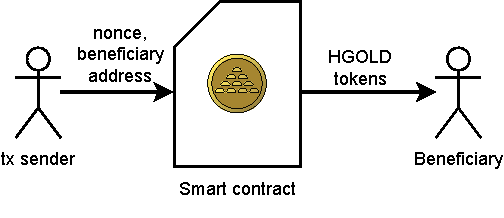
\includegraphics{figures/tx-v2.drawio.pdf}
    \caption{Hashmaxxing: tx sender (miner a.k.a. hashmaxxer) sends the nonce along with the beneficiary address to the smart contract. The contract verifies the nonce, and if it is correct, mints a given number of tokens to beneficiary. Beneficiary can be any valid address, including the same address as \texttt{tx.sender}.}
    \label{fig:hashmaxxxing}
\end{figure}


\begin{algorithm}[H]
\caption{Simplified Hashmaxxing algorithm}\label{alg:hashmaxxing}
\begin{lstlisting}
new_hash = keccak256(
        keccak256(
            keccak256(noncecount[beneficiary]) // 32 bytes
            + keccak256(chainId)               // 32 bytes
            + nonce                            // 32 bytes
            + beneficiary                      // 20 bytes
        )
);

noncecount[beneficiary] = noncecount[beneficiary] + 1;

if (new_hash > current_target_hash) {
    mint_rewards(beneficary);
    update_target_hash_if_necessary();
}
\end{lstlisting}

\end{algorithm}
\subsubsection{Updating the target hash}
The target hash is initially set to
\begin{equation*}
\texttt{0xffffff000000000000000000000000000000000000000000000000000b00b1e5},
\end{equation*}
which is chosen in such way, that a single Macbook Air M1 can find a correct nonce in about 10 seconds. The target hash is incremented based on the number of nonces accepted by the contract. After every \rewardPerNonce~nonces, the target hash is incremented in the following way: most significant byte less than $255$ is incremented by $8$. For example the next target hash after the initial target hash will be
\begin{equation*}
\texttt{0xffffff080000000000000000000000000000000000000000000000000b00b1e5},
\end{equation*}
and the next will be
\begin{equation*}
\texttt{0xffffff180000000000000000000000000000000000000000000000000b00b1e5},
\end{equation*}
and so on, until the target hash becomes
\begin{equation*}
\texttt{0xffffffffffffffffffffffffffffffffffffffffffffffffffffffffffffffff}.
\end{equation*}
This way we create a mechanism that ensures a hard cap on the number of tokens in existence, and also makes hashmaxxing exponentially harder over time. Target hash is updated after every \incrementPeriodNonces~nonces and every correct nonce is worth \rewardPerNonce~tokens, so the target hash is updated after every
\tokensPerHashUpdate~tokens created.
\subsection{Tokenomics}
Hashgold is deployed on two chains: Ethereum and Arbitrum. On each of these chains there will be \totalNumberofIncremensPerChain~target hash updates, and between each such hash update \tokensPerHashUpdate~tokens are created. 
This way, the absolute theoretical maximum of tokens in existence is $2\times$\tokenHardCapPerChain=\tokenHardCapTotal. In practice however this number will never be reached, due to the exponential difficulty of mining tokens and the fact that token mining will be stopped after \tokenMiningStopped.

\newpage
\section{Benchmarks}

We perfomed benchmarks of the Hashmaxxing algorithm using the rust hashmaxxing software on an Apple™ Macbook Air with M1 chip and on a server with AMD EPYC™ 7742 CPUs, for different target hashes. As expected, in all tests we find that the effort needed to find a correct nonce increases exponentially with the target hash increments, see Fig \ref{fig:measurements}.
\newcommand{\thisfigurewidth}{0.5}
\begin{figure}[H]
    \centering
    \begin{tabular}{cc}
      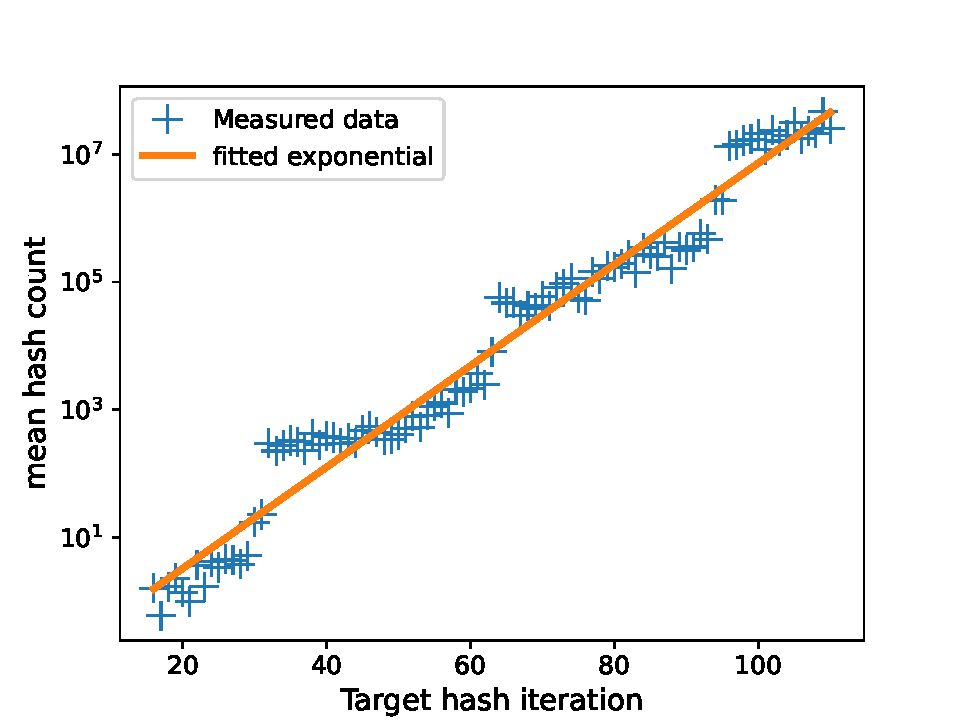
\includegraphics[width=\thisfigurewidth\textwidth]{figures/m1_hashcount.pdf} & 
      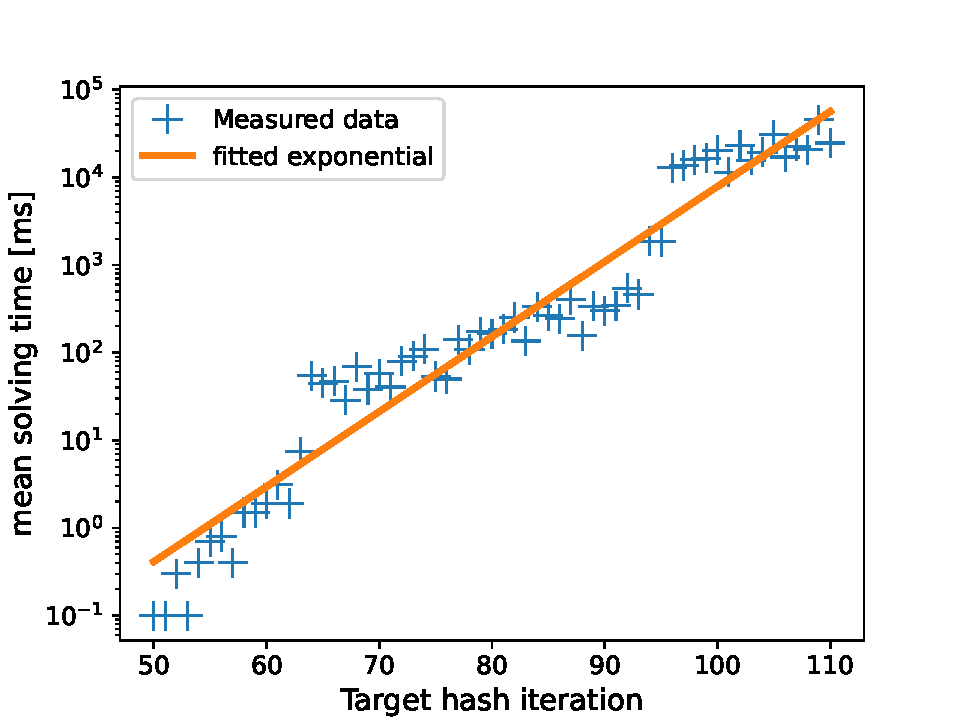
\includegraphics[width=\thisfigurewidth\textwidth]{figures/m1_solving_time.pdf} \\
      (a) & (b) \\[6.5pt]
      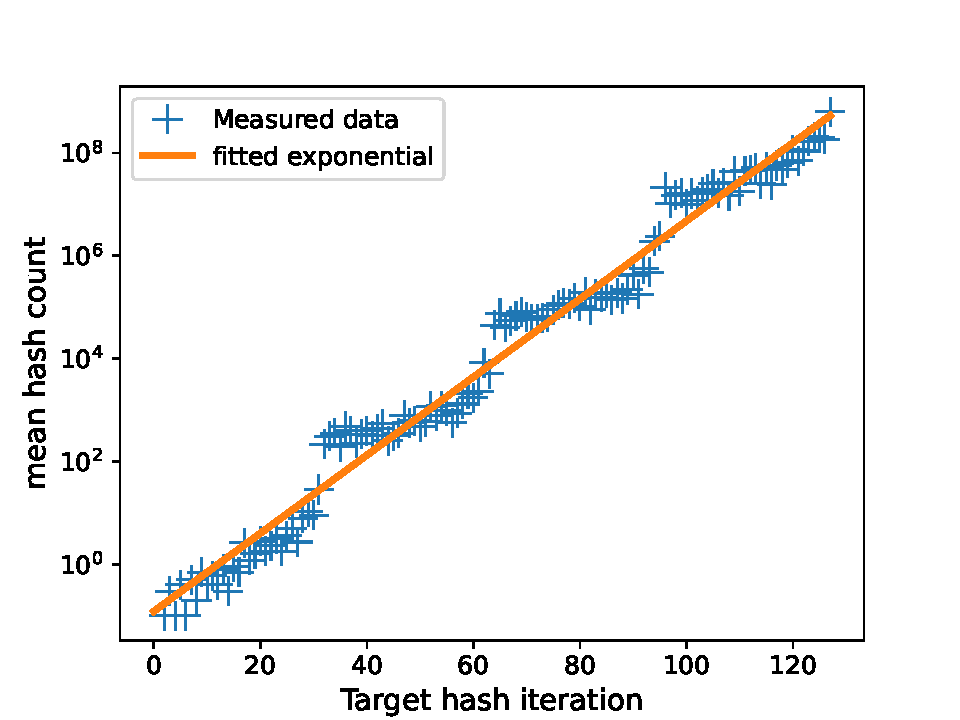
\includegraphics[width=\thisfigurewidth\textwidth]{figures/amd_hashcount.pdf} & 
      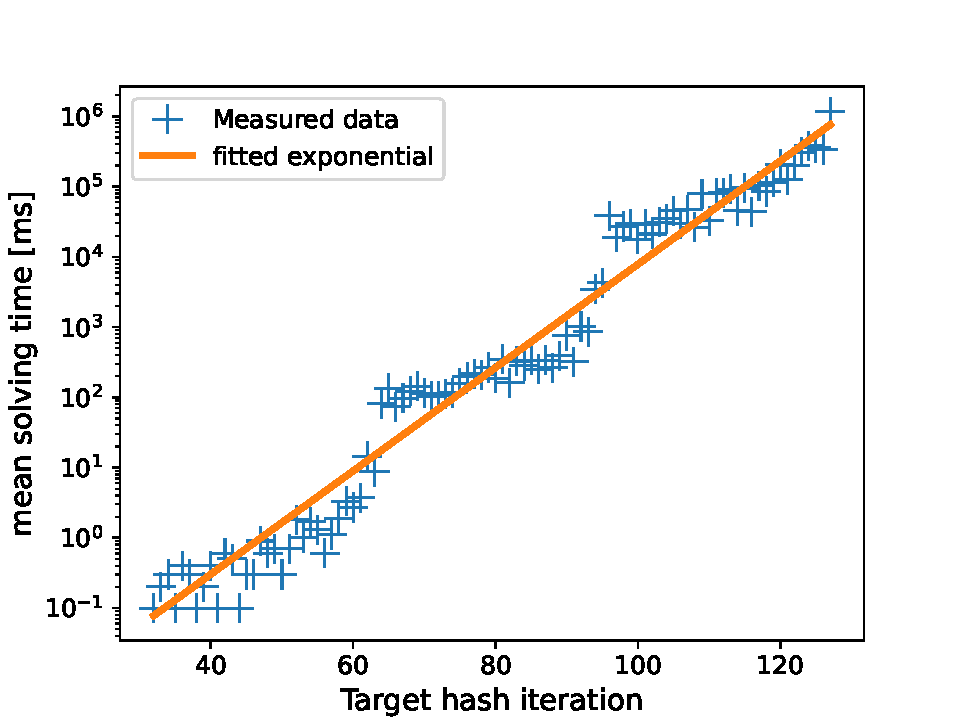
\includegraphics[width=\thisfigurewidth\textwidth]{figures/amd_solving_time.pdf} \\
      (c) & (d) \\[6.5pt]
    \end{tabular}
    \caption{Benchmark results and exponential fits. (a) average number of hashes needed to find a nonce on a Macbook Air with M1 chip, (b) average time in milliseconds needed to find a nonce on a Macbook Air with M1 chip, (c) average number of hashes needed to find a nonce on an AMD EPYC™ 7742 CPU, (d) average time in milliseconds needed to find a nonce on an AMD EPYC™ 7742 CPU.}
    \label{fig:measurements}
\end{figure}

Tables \ref{tab:m1_1}-\ref{tab:amd_3} contain the benchmarking data we measured on the CPUs and used to create Fig. \ref{fig:measurements}.

\begin{table}[H]
    \centering
    \begin{tabular}{|c|c|c|c|c|} \hline
    target hash  & $\mathbb{E}(k)$ & $\sigma(k) $ & $\mathbb{E}(t)$ [ms] & $\sigma(t)$ [ms] \\ \hline
    0x0000000000...b00b1e5 &        0.0000 &        0.0000 &         0.0000 &        0.0000 \\ \hline
0x0800000000...b00b1e5 &        0.1000 &        0.3162 &         0.0000 &        0.0000 \\ \hline
0x1000000000...b00b1e5 &        0.0000 &        0.0000 &         0.0000 &        0.0000 \\ \hline
0x1800000000...b00b1e5 &        0.0000 &        0.0000 &         0.0000 &        0.0000 \\ \hline
0x2000000000...b00b1e5 &        0.2000 &        0.6325 &         0.0000 &        0.0000 \\ \hline
0x2800000000...b00b1e5 &        0.3000 &        0.4830 &         0.0000 &        0.0000 \\ \hline
0x3000000000...b00b1e5 &        0.0000 &        0.0000 &         0.0000 &        0.0000 \\ \hline
0x3800000000...b00b1e5 &        0.4000 &        0.8433 &         0.0000 &        0.0000 \\ \hline
0x4000000000...b00b1e5 &        0.1000 &        0.3162 &         0.0000 &        0.0000 \\ \hline
0x4800000000...b00b1e5 &        0.1000 &        0.3162 &         0.0000 &        0.0000 \\ \hline
0x5000000000...b00b1e5 &        0.3000 &        0.6749 &         0.0000 &        0.0000 \\ \hline
0x5800000000...b00b1e5 &        0.4000 &        0.6992 &         0.0000 &        0.0000 \\ \hline
0x6000000000...b00b1e5 &        0.6000 &        0.9661 &         0.0000 &        0.0000 \\ \hline
0x6800000000...b00b1e5 &        0.3000 &        0.4830 &         0.0000 &        0.0000 \\ \hline
0x7000000000...b00b1e5 &        1.3000 &        1.3375 &         0.0000 &        0.0000 \\ \hline
0x7800000000...b00b1e5 &        0.5000 &        0.9718 &         0.0000 &        0.0000 \\ \hline
0x8000000000...b00b1e5 &        1.6000 &        2.0656 &         0.0000 &        0.0000 \\ \hline
0x8800000000...b00b1e5 &        0.6000 &        0.6992 &         0.0000 &        0.0000 \\ \hline
0x9000000000...b00b1e5 &        1.7000 &        1.4944 &         0.0000 &        0.0000 \\ \hline
0x9800000000...b00b1e5 &        2.3000 &        2.4060 &         0.0000 &        0.0000 \\ \hline
0xa000000000...b00b1e5 &        1.4000 &        1.3499 &         0.0000 &        0.0000 \\ \hline
0xa800000000...b00b1e5 &        1.0000 &        0.9428 &         0.0000 &        0.0000 \\ \hline
0xb000000000...b00b1e5 &        3.7000 &        2.1108 &         0.0000 &        0.0000 \\ \hline
0xb800000000...b00b1e5 &        1.7000 &        1.3375 &         0.0000 &        0.0000 \\ \hline
0xc000000000...b00b1e5 &        4.2000 &        3.7059 &         0.0000 &        0.0000 \\ \hline
0xc800000000...b00b1e5 &        3.4000 &        2.5906 &         0.0000 &        0.0000 \\ \hline
0xd000000000...b00b1e5 &        4.6000 &        5.1897 &         0.0000 &        0.0000 \\ \hline
0xd800000000...b00b1e5 &        4.4000 &        6.3805 &         0.0000 &        0.0000 \\ \hline
0xe000000000...b00b1e5 &        3.8000 &        4.3153 &         0.0000 &        0.0000 \\ \hline
0xe800000000...b00b1e5 &        5.2000 &        4.9171 &         0.0000 &        0.0000 \\ \hline
0xf000000000...b00b1e5 &       17.4000 &       21.4900 &         0.0000 &        0.0000 \\ \hline
0xf800000000...b00b1e5 &       23.0000 &       21.0766 &         0.0000 &        0.0000 \\ \hline
0xff00000000...b00b1e5 &      299.1000 &      176.3056 &         0.0000 &        0.0000 \\ \hline
0xff08000000...b00b1e5 &      226.3000 &      228.1155 &         0.0000 &        0.0000 \\ \hline
0xff10000000...b00b1e5 &      275.8000 &      294.1118 &         0.0000 &        0.0000 \\ \hline
0xff18000000...b00b1e5 &      330.9000 &      484.6780 &         0.1000 &        0.3162 \\ \hline
0xff20000000...b00b1e5 &      317.8000 &      188.2279 &         0.0000 &        0.0000 \\ \hline
0xff28000000...b00b1e5 &      232.9000 &      205.4629 &         0.0000 &        0.0000 \\ \hline
0xff30000000...b00b1e5 &      419.8000 &      537.7715 &         0.1000 &        0.3162 \\ \hline
0xff38000000...b00b1e5 &      284.2000 &      202.0895 &         0.0000 &        0.0000 \\ \hline
0xff40000000...b00b1e5 &      387.7000 &      261.6992 &         0.0000 &        0.0000 \\ \hline
0xff48000000...b00b1e5 &      368.4000 &      249.2001 &         0.0000 &        0.0000 \\ \hline
0xff50000000...b00b1e5 &      299.5000 &      204.3702 &         0.0000 &        0.0000 \\ \hline
 \end{tabular}
    \caption{M1 part 1}
    \label{tab:m1_1}
\end{table}

\begin{table}[H]
    \centering
    \begin{tabular}{|c|c|c|c|c|} \hline
    target hash  & $\mathbb{E}(k)$ & $\sigma(k) $ & $\mathbb{E}(t)$ [ms] & $\sigma(t)$ [ms] \\ \hline
    0xff58000000...b00b1e5 &      357.9000 &      382.9956 &         0.1000 &        0.3162 \\ \hline
0xff60000000...b00b1e5 &      304.3000 &      324.0172 &         0.0000 &        0.0000 \\ \hline
0xff68000000...b00b1e5 &      479.3000 &      398.8275 &         0.2000 &        0.4216 \\ \hline
0xff70000000...b00b1e5 &      547.8000 &      607.6296 &         0.2000 &        0.4216 \\ \hline
0xff78000000...b00b1e5 &      442.7000 &      301.2865 &         0.1000 &        0.3162 \\ \hline
0xff80000000...b00b1e5 &      339.8000 &      379.1874 &         0.1000 &        0.3162 \\ \hline
0xff88000000...b00b1e5 &      347.8000 &      393.7441 &         0.1000 &        0.3162 \\ \hline
0xff90000000...b00b1e5 &      404.1000 &      448.9354 &         0.1000 &        0.3162 \\ \hline
0xff98000000...b00b1e5 &      513.0000 &      492.2472 &         0.1000 &        0.3162 \\ \hline
0xffa0000000...b00b1e5 &      793.2000 &      847.1994 &         0.3000 &        0.6749 \\ \hline
0xffa8000000...b00b1e5 &      534.3000 &      541.6309 &         0.1000 &        0.3162 \\ \hline
0xffb0000000...b00b1e5 &      818.6000 &     1005.6472 &         0.4000 &        0.9661 \\ \hline
0xffb8000000...b00b1e5 &     1143.0000 &     1017.7993 &         0.7000 &        0.8233 \\ \hline
0xffc0000000...b00b1e5 &     1276.7000 &     1017.5443 &         0.8000 &        1.0328 \\ \hline
0xffc8000000...b00b1e5 &      886.1000 &      874.9747 &         0.4000 &        0.6992 \\ \hline
0xffd0000000...b00b1e5 &     2078.1000 &     2442.9170 &         1.5000 &        2.1731 \\ \hline
0xffd8000000...b00b1e5 &     1910.1000 &     1559.9636 &         1.5000 &        1.5092 \\ \hline
0xffe0000000...b00b1e5 &     2185.6000 &     2274.0737 &         1.9000 &        2.2336 \\ \hline
0xffe8000000...b00b1e5 &     3737.7000 &     2754.2146 &         3.1000 &        2.7264 \\ \hline
0xfff0000000...b00b1e5 &     2457.7000 &     2541.6149 &         1.9000 &        2.3310 \\ \hline
0xfff8000000...b00b1e5 &     8052.9000 &    10955.8438 &         7.4000 &       10.5641 \\ \hline
0xffff000000...b00b1e5 &    57233.9000 &    51344.0133 &        54.7000 &       49.6612 \\ \hline
0xffff080000...b00b1e5 &    46988.3000 &    32388.3959 &        44.9000 &       31.0285 \\ \hline
0xffff100000...b00b1e5 &    47792.4000 &    51234.6532 &        47.0000 &       50.5129 \\ \hline
0xffff180000...b00b1e5 &    30320.8000 &    25531.9665 &        28.8000 &       24.6928 \\ \hline
0xffff200000...b00b1e5 &    42274.6000 &    42683.0719 &        69.2000 &       65.8429 \\ \hline
0xffff280000...b00b1e5 &    38907.6000 &    45678.1507 &        37.6000 &       45.8650 \\ \hline
0xffff300000...b00b1e5 &    59464.6000 &    68559.7647 &        57.3000 &       66.9744 \\ \hline
0xffff380000...b00b1e5 &    42577.7000 &    46386.0088 &        40.6000 &       44.7988 \\ \hline
0xffff400000...b00b1e5 &    83155.8000 &    93872.7655 &        79.9000 &       90.4771 \\ \hline
0xffff480000...b00b1e5 &    94449.7000 &    68853.8725 &        90.7000 &       66.4012 \\ \hline
0xffff500000...b00b1e5 &   113586.4000 &   125259.7631 &       109.4000 &      121.1172 \\ \hline
0xffff580000...b00b1e5 &    56053.5000 &    73681.8122 &        53.5000 &       70.9260 \\ \hline
0xffff600000...b00b1e5 &    52288.1000 &    48799.0571 &        50.1000 &       47.0943 \\ \hline
0xffff680000...b00b1e5 &   145321.8000 &    97332.9590 &       139.7000 &       93.8688 \\ \hline
0xffff700000...b00b1e5 &   112950.3000 &    81856.1993 &       108.8000 &       79.7479 \\ \hline
0xffff780000...b00b1e5 &   180284.6000 &    73720.0260 &       173.4000 &       70.7565 \\ \hline
0xffff800000...b00b1e5 &   169771.2000 &   139975.8842 &       164.2000 &      136.2936 \\ \hline
0xffff880000...b00b1e5 &   192866.5000 &   182177.4010 &       185.7000 &      176.2259 \\ \hline
0xffff900000...b00b1e5 &   261789.4000 &   219321.2979 &       252.2000 &      211.9129 \\ \hline
 \end{tabular}
    \caption{M1 part 2}
    \label{tab:m1_2}
\end{table}



\begin{table}[H]
    \centering
    \begin{tabular}{|c|c|c|c|c|} \hline
    target hash  & $\mathbb{E}(k)$ & $\sigma(k) $ & $\mathbb{E}(t)$ [ms] & $\sigma(t)$ [ms] \\ \hline
    
0xffff980000...b00b1e5 &   141419.3000 &   162581.8159 &       135.9000 &      156.6209 \\ \hline
0xffffa00000...b00b1e5 &   343411.8000 &   468316.3227 &       332.6000 &      451.6326 \\ \hline
0xffffa80000...b00b1e5 &   272762.0000 &   297238.0381 &       262.8000 &      286.4661 \\ \hline
0xffffb00000...b00b1e5 &   252887.9000 &   107113.8918 &       243.3000 &      103.1838 \\ \hline
0xffffb80000...b00b1e5 &   416602.3000 &   470681.4057 &       401.4000 &      453.9193 \\ \hline
0xffffc00000...b00b1e5 &   161727.9000 &   177162.2591 &       155.5000 &      170.8178 \\ \hline
0xffffc80000...b00b1e5 &   350480.7000 &   290516.0550 &       337.9000 &      280.7096 \\ \hline
0xffffd00000...b00b1e5 &   313978.6000 &   196239.6396 &       302.0000 &      189.1543 \\ \hline
0xffffd80000...b00b1e5 &   354235.9000 &   369426.2711 &       341.1000 &      356.1930 \\ \hline
0xffffe00000...b00b1e5 &   566150.9000 &   417088.3179 &       545.2000 &      401.9618 \\ \hline
0xffffe80000...b00b1e5 &   469943.6000 &   391102.5292 &       460.9000 &      379.5613 \\ \hline
0xfffff00000...b00b1e5 &  1937844.7000 &  1835596.3125 &      1869.8000 &     1774.1910 \\ \hline
0xfffff80000...b00b1e5 &  1897883.3000 &  1283729.2209 &      1833.7000 &     1236.1626 \\ \hline
0xffffff0000...b00b1e5 & 13318781.8000 &  8605073.8175 &     12872.4000 &     8308.2591 \\ \hline
0xffffff0800...b00b1e5 & 14110975.7000 & 13143622.0721 &     13633.4000 &    12705.6558 \\ \hline
0xffffff1000...b00b1e5 & 16461097.3000 & 17667646.7655 &     15929.6000 &    17120.0902 \\ \hline
0xffffff1800...b00b1e5 & 17127336.7000 & 18367801.2597 &     16599.5000 &    17797.9577 \\ \hline
0xffffff2000...b00b1e5 & 20956241.6000 &  9600384.9595 &     20316.3000 &     9310.1935 \\ \hline
0xffffff2800...b00b1e5 & 11730598.3000 &  8183260.3529 &     11406.4000 &     7969.4622 \\ \hline
0xffffff3000...b00b1e5 & 23877718.1000 & 19702863.7984 &     23192.4000 &    19127.9219 \\ \hline
0xffffff3800...b00b1e5 & 16142472.2000 & 18647230.3415 &     15690.5000 &    18129.6404 \\ \hline
0xffffff4000...b00b1e5 & 19943237.6000 & 20487399.8308 &     19400.5000 &    19933.7991 \\ \hline
0xffffff4800...b00b1e5 & 31574051.1000 & 22763341.6808 &     30695.3000 &    22131.2361 \\ \hline
0xffffff5000...b00b1e5 & 17560495.2000 & 19104704.7562 &     17075.9000 &    18554.7347 \\ \hline
0xffffff5800...b00b1e5 & 23173131.9000 & 26412213.5635 &     22564.1000 &    25737.0254 \\ \hline
0xffffff6000...b00b1e5 & 21337645.6000 & 14264328.0630 &     20737.7000 &    13870.6749 \\ \hline
0xffffff6800...b00b1e5 & 46607821.0000 & 33683525.4612 &     45317.2000 &    32713.3751 \\ \hline
0xffffff7000...b00b1e5 & 25358568.8000 & 24168956.1925 &     24645.3000 &    23505.4801 \\ \hline
    \end{tabular}
    \caption{M1 part 3}
    \label{tab:m1_3}
\end{table}

\begin{table}[H]
    \centering
    \begin{tabular}{|c|c|c|c|c|} \hline
    target hash  & $\mathbb{E}(k)$ & $\sigma(k) $ & $\mathbb{E}(t)$ [ms] & $\sigma(t)$ [ms] \\ \hline
    0x000000000...b00b1e5 &         0.0000 &         0.0000 &         0.0000 &        0.0000 \\ \hline
0x080000000...b00b1e5 &         0.0000 &         0.0000 &         0.0000 &        0.0000 \\ \hline
0x100000000...b00b1e5 &         0.1000 &         0.3162 &         0.0000 &        0.0000 \\ \hline
0x180000000...b00b1e5 &         0.3000 &         0.6749 &         0.0000 &        0.0000 \\ \hline
0x200000000...b00b1e5 &         0.1000 &         0.3162 &         0.0000 &        0.0000 \\ \hline
0x280000000...b00b1e5 &         0.4000 &         0.5164 &         0.0000 &        0.0000 \\ \hline
0x300000000...b00b1e5 &         0.1000 &         0.3162 &         0.0000 &        0.0000 \\ \hline
0x380000000...b00b1e5 &         0.5000 &         0.7071 &         0.0000 &        0.0000 \\ \hline
0x400000000...b00b1e5 &         0.2000 &         0.4216 &         0.0000 &        0.0000 \\ \hline
0x480000000...b00b1e5 &         0.7000 &         0.6749 &         0.0000 &        0.0000 \\ \hline
0x500000000...b00b1e5 &         0.4000 &         0.6992 &         0.0000 &        0.0000 \\ \hline
0x580000000...b00b1e5 &         0.6000 &         0.8433 &         0.0000 &        0.0000 \\ \hline
0x600000000...b00b1e5 &         0.4000 &         0.6992 &         0.0000 &        0.0000 \\ \hline
0x680000000...b00b1e5 &         0.8000 &         1.0328 &         0.0000 &        0.0000 \\ \hline
0x700000000...b00b1e5 &         0.3000 &         0.6749 &         0.0000 &        0.0000 \\ \hline
0x780000000...b00b1e5 &         0.9000 &         0.9944 &         0.0000 &        0.0000 \\ \hline
0x800000000...b00b1e5 &         0.7000 &         1.1595 &         0.0000 &        0.0000 \\ \hline
0x880000000...b00b1e5 &         2.6000 &         4.0607 &         0.0000 &        0.0000 \\ \hline
0x900000000...b00b1e5 &         1.2000 &         0.7888 &         0.0000 &        0.0000 \\ \hline
0x980000000...b00b1e5 &         1.6000 &         1.5776 &         0.0000 &        0.0000 \\ \hline
0xa00000000...b00b1e5 &         2.8000 &         3.7947 &         0.0000 &        0.0000 \\ \hline
0xa80000000...b00b1e5 &         1.8000 &         2.1499 &         0.0000 &        0.0000 \\ \hline
0xb00000000...b00b1e5 &         2.3000 &         1.9465 &         0.0000 &        0.0000 \\ \hline
0xb80000000...b00b1e5 &         3.1000 &         2.9231 &         0.0000 &        0.0000 \\ \hline
0xc00000000...b00b1e5 &         1.8000 &         1.2293 &         0.0000 &        0.0000 \\ \hline
0xc80000000...b00b1e5 &         3.6000 &         3.0623 &         0.0000 &        0.0000 \\ \hline
0xd00000000...b00b1e5 &         5.0000 &         4.5216 &         0.0000 &        0.0000 \\ \hline
0xd80000000...b00b1e5 &         2.7000 &         3.3350 &         0.0000 &        0.0000 \\ \hline
0xe00000000...b00b1e5 &         7.8000 &         4.5412 &         0.0000 &        0.0000 \\ \hline
0xe80000000...b00b1e5 &        10.6000 &         6.8346 &         0.0000 &        0.0000 \\ \hline
0xf00000000...b00b1e5 &         9.0000 &         7.5130 &         0.0000 &        0.0000 \\ \hline
0xf80000000...b00b1e5 &        28.3000 &        28.5542 &         0.0000 &        0.0000 \\ \hline
0xff0000000...b00b1e5 &       215.2000 &       213.9869 &         0.1000 &        0.3162 \\ \hline
0xff0800000...b00b1e5 &       309.1000 &       278.8219 &         0.2000 &        0.4216 \\ \hline
0xff1000000...b00b1e5 &       354.7000 &       320.8994 &         0.3000 &        0.4830 \\ \hline
0xff1800000...b00b1e5 &       195.3000 &       181.6713 &         0.1000 &        0.3162 \\ \hline
0xff2000000...b00b1e5 &       477.2000 &       470.2559 &         0.4000 &        0.8433 \\ \hline
0xff2800000...b00b1e5 &       394.4000 &       350.5260 &         0.3000 &        0.4830 \\ \hline
0xff3000000...b00b1e5 &       224.0000 &       199.2374 &         0.1000 &        0.3162 \\ \hline
0xff3800000...b00b1e5 &       338.4000 &       283.2510 &         0.2000 &        0.4216 \\ \hline
0xff4000000...b00b1e5 &       396.0000 &       354.3507 &         0.4000 &        0.5164 \\ \hline
0xff4800000...b00b1e5 &       315.1000 &       218.0802 &         0.1000 &        0.3162 \\ \hline
0xff5000000...b00b1e5 &       432.7000 &       585.3649 &         0.6000 &        0.9661 \\ \hline
    \end{tabular}
    \caption{AMD part 1}
    \label{tab:amd_1}
\end{table}

\begin{table}[H]
    \centering
    \begin{tabular}{|c|c|c|c|c|} \hline
    target hash  & $\mathbb{E}(k)$ & $\sigma(k) $ & $\mathbb{E}(t)$ [ms] & $\sigma(t)$ [ms] \\ \hline
    0xff5800000...b00b1e5 &       540.5000 &       444.6877 &         0.5000 &        0.7071 \\ \hline
0xff6000000...b00b1e5 &       253.0000 &       246.1991 &         0.1000 &        0.3162 \\ \hline
0xff6800000...b00b1e5 &       313.9000 &       353.9763 &         0.3000 &        0.4830 \\ \hline
0xff7000000...b00b1e5 &       350.9000 &       285.8517 &         0.3000 &        0.4830 \\ \hline
0xff7800000...b00b1e5 &       789.7000 &       861.1474 &         0.9000 &        1.6633 \\ \hline
0xff8000000...b00b1e5 &       566.7000 &       560.2654 &         0.6000 &        1.0750 \\ \hline
0xff8800000...b00b1e5 &       618.1000 &       530.9956 &         0.7000 &        0.9487 \\ \hline
0xff9000000...b00b1e5 &       472.7000 &       307.0472 &         0.3000 &        0.4830 \\ \hline
0xff9800000...b00b1e5 &       584.7000 &       334.1168 &         0.7000 &        0.6749 \\ \hline
0xffa000000...b00b1e5 &      1167.7000 &      1122.5245 &         1.8000 &        2.0976 \\ \hline
0xffa800000...b00b1e5 &       764.5000 &       363.9064 &         1.0000 &        0.8165 \\ \hline
0xffb000000...b00b1e5 &      1206.2000 &       996.9248 &         1.7000 &        1.8288 \\ \hline
0xffb800000...b00b1e5 &       970.7000 &       847.2341 &         1.3000 &        1.3375 \\ \hline
0xffc000000...b00b1e5 &       560.2000 &       398.8993 &         0.6000 &        0.6992 \\ \hline
0xffc800000...b00b1e5 &       861.1000 &       685.1004 &         1.1000 &        1.2867 \\ \hline
0xffd000000...b00b1e5 &      1305.9000 &       938.9964 &         1.9000 &        1.7920 \\ \hline
0xffd800000...b00b1e5 &      2049.3000 &      2253.5551 &         3.3000 &        3.9735 \\ \hline
0xffe000000...b00b1e5 &      1740.1000 &      2340.3176 &         2.7000 &        4.2960 \\ \hline
0xffe800000...b00b1e5 &      2319.5000 &      2199.6745 &         3.7000 &        3.7727 \\ \hline
0xfff000000...b00b1e5 &      8346.5000 &      8335.5767 &        14.4000 &       14.9012 \\ \hline
0xfff800000...b00b1e5 &      5093.6000 &      4589.7728 &         8.7000 &        8.2603 \\ \hline
0xffff00000...b00b1e5 &     44846.2000 &     36883.5249 &        80.5000 &       66.6804 \\ \hline
0xffff08000...b00b1e5 &     75100.6000 &     40710.0714 &       134.7000 &       73.2637 \\ \hline
0xffff10000...b00b1e5 &     40896.4000 &     28169.6211 &        73.2000 &       50.6750 \\ \hline
0xffff18000...b00b1e5 &     54393.8000 &     52335.8164 &        97.6000 &       94.2399 \\ \hline
0xffff20000...b00b1e5 &     68093.0000 &     48667.1164 &       122.1000 &       87.5715 \\ \hline
0xffff28000...b00b1e5 &     80573.4000 &     73653.3179 &       144.5000 &      132.5940 \\ \hline
0xffff30000...b00b1e5 &     63945.0000 &     57096.7891 &       114.7000 &      103.4817 \\ \hline
0xffff38000...b00b1e5 &     57998.5000 &     81449.1599 &       104.1000 &      146.5874 \\ \hline
0xffff40000...b00b1e5 &     59092.4000 &     55654.9843 &       105.9000 &      100.2103 \\ \hline
0xffff48000...b00b1e5 &     62604.8000 &     57813.7979 &       112.4000 &      104.1881 \\ \hline
0xffff50000...b00b1e5 &     64963.8000 &     53997.0472 &       116.5000 &       97.1302 \\ \hline
0xffff58000...b00b1e5 &     88192.7000 &     77423.3106 &       158.5000 &      139.2035 \\ \hline
0xffff60000...b00b1e5 &    108642.4000 &     79414.4133 &       195.5000 &      143.2940 \\ \hline
0xffff68000...b00b1e5 &    119904.4000 &    118635.3072 &       215.4000 &      213.8365 \\ \hline
0xffff70000...b00b1e5 &    116141.6000 &    144913.2697 &       208.6000 &      260.9143 \\ \hline
0xffff78000...b00b1e5 &    148085.8000 &    146302.9797 &       266.1000 &      263.1394 \\ \hline
0xffff80000...b00b1e5 &    103791.3000 &     87025.9021 &       186.3000 &      156.7468 \\ \hline
0xffff88000...b00b1e5 &    194147.2000 &     88481.6693 &       349.0000 &      159.3410 \\ \hline
0xffff90000...b00b1e5 &     89276.2000 &    108880.3010 &       160.3000 &      196.1032 \\ \hline
0xffff98000...b00b1e5 &    182965.8000 &    234044.4978 &       329.0000 &      421.1666 \\ \hline
0xffffa0000...b00b1e5 &    156213.0000 &    139686.0204 &       280.9000 &      251.8864 \\ \hline
0xffffa8000...b00b1e5 &    187430.3000 &    252817.8469 &       336.7000 &      455.1249 \\ \hline
0xffffb0000...b00b1e5 &    139696.7000 &    145773.6257 &       251.1000 &      262.2939 \\ \hline
    \end{tabular}
    \caption{AMD part 2}
    \label{tab:amd_2}
\end{table}

\begin{table}[H]
    \centering
    \begin{tabular}{|c|c|c|c|c|} \hline
    target hash  & $\mathbb{E}(k)$ & $\sigma(k) $ & $\mathbb{E}(t)$ [ms] & $\sigma(t)$ [ms] \\ \hline
    0xffffb8000...b00b1e5 &    188487.2000 &    205919.2111 &       339.0000 &      370.7272 \\ \hline
0xffffc0000...b00b1e5 &    147754.0000 &    148595.9419 &       265.3000 &      267.3579 \\ \hline
0xffffc8000...b00b1e5 &    217976.5000 &    246670.0897 &       392.0000 &      444.1116 \\ \hline
0xffffd0000...b00b1e5 &    421568.7000 &    358833.6118 &       758.1000 &      645.6281 \\ \hline
0xffffd8000...b00b1e5 &    179499.9000 &    132069.9668 &       322.7000 &      237.6884 \\ \hline
0xffffe0000...b00b1e5 &    566541.2000 &    512566.7710 &      1019.3000 &      922.3528 \\ \hline
0xffffe8000...b00b1e5 &    477459.4000 &    419580.0773 &       858.9000 &      755.2319 \\ \hline
0xfffff0000...b00b1e5 &   1912030.7000 &   2184809.2852 &      3440.9000 &     3931.7243 \\ \hline
0xfffff8000...b00b1e5 &   2376509.8000 &   2481948.4281 &      4279.5000 &     4467.4432 \\ \hline
0xffffff000...b00b1e5 &  21486445.5000 &   9491597.3216 &     38678.1000 &    17089.1058 \\ \hline
0xffffff080...b00b1e5 &  10593226.2000 &   6210012.3285 &     19071.3000 &    11179.5759 \\ \hline
0xffffff100...b00b1e5 &  15079070.3000 &  13058176.6272 &     27142.7000 &    23507.4024 \\ \hline
0xffffff180...b00b1e5 &  16312876.2000 &  18387866.7940 &     29371.0000 &    33099.7172 \\ \hline
0xffffff200...b00b1e5 &   9913930.5000 &   8789908.4892 &     17841.2000 &    15822.5846 \\ \hline
0xffffff280...b00b1e5 &  16220390.8000 &  21635050.1824 &     29192.6000 &    38922.9919 \\ \hline
0xffffff300...b00b1e5 &  11771356.4000 &  11737164.7967 &     21176.4000 &    21113.5629 \\ \hline
0xffffff380...b00b1e5 &  17223865.9000 &  21501572.7888 &     31010.9000 &    38694.6999 \\ \hline
0xffffff400...b00b1e5 &  19365033.6000 &  23997971.2424 &     34858.0000 &    43194.0122 \\ \hline
0xffffff480...b00b1e5 &  25024493.9000 &  29961724.5655 &     45054.6000 &    53926.4718 \\ \hline
0xffffff500...b00b1e5 &  16430705.1000 &  12811609.0536 &     29578.0000 &    23062.3093 \\ \hline
0xffffff580...b00b1e5 &  25949395.8000 &  34260902.4714 &     46713.1000 &    61667.1997 \\ \hline
0xffffff600...b00b1e5 &  14741662.4000 &  13302872.9177 &     26531.1000 &    23943.2628 \\ \hline
0xffffff680...b00b1e5 &  43721412.5000 &  51112239.7266 &     78688.2000 &    91978.1163 \\ \hline
0xffffff700...b00b1e5 &  18056553.7000 &  10164951.5784 &     32504.9000 &    18300.3520 \\ \hline
0xffffff780...b00b1e5 &  44510497.7000 &  44223567.8203 &     80149.4000 &    79607.0098 \\ \hline
0xffffff800...b00b1e5 &  45697626.9000 &  35777392.1517 &     82253.4000 &    64401.2592 \\ \hline
0xffffff880...b00b1e5 &  51111026.3000 &  75141671.6992 &     92015.3000 &   135305.4488 \\ \hline
0xffffff900...b00b1e5 &  25258048.9000 &  23435909.7131 &     45534.1000 &    42172.5247 \\ \hline
0xffffff980...b00b1e5 &  53100895.7000 &  30730131.1177 &     95619.4000 &    55360.3205 \\ \hline
0xffffffa00...b00b1e5 &  24290830.0000 &  22851043.9569 &     43741.2000 &    41143.1731 \\ \hline
0xffffffa80...b00b1e5 &  56925460.1000 &  50747390.2781 &    102568.0000 &    91428.4544 \\ \hline
0xffffffb00...b00b1e5 &  47486028.8000 &  57185053.1094 &     85482.9000 &   102961.8334 \\ \hline
0xffffffb80...b00b1e5 &  64586214.3000 &  48833072.0631 &    116266.1000 &    87900.4087 \\ \hline
0xffffffc00...b00b1e5 & 114668240.6000 &  98772976.6111 &    206429.9000 &   177818.4960 \\ \hline
0xffffffc80...b00b1e5 &  69884977.1000 &  63711701.8537 &    125883.1000 &   114767.9633 \\ \hline
0xffffffd00...b00b1e5 & 109130350.2000 &  88302151.3254 &    197042.1000 &   159167.7096 \\ \hline
0xffffffd80...b00b1e5 & 167418702.6000 & 185092851.5179 &    308348.0000 &   341336.9993 \\ \hline
0xffffffe00...b00b1e5 & 206806907.3000 & 228491083.6649 &    381045.6000 &   421629.7122 \\ \hline
0xffffffe80...b00b1e5 & 196709377.0000 & 192985177.4848 &    361236.0000 &   354834.3142 \\ \hline
0xfffffff00...b00b1e5 & 184554527.4000 & 216867907.8177 &    338558.6000 &   397074.4479 \\ \hline
0xfffffff80...b00b1e5 & 636269011.1000 & 786413959.7945 &   1170823.1000 &  1452144.1791 \\ \hline

\end{tabular}
    \caption{AMD part 3}
    \label{tab:amd_3}
\end{table}

\end{document}
